\documentclass[aspectratio=169]{beamer}
\usepackage{lmodern}
\usetheme{Madrid}
%\usecolortheme{giantoak}
\newcommand*\oldmacro{}
\let\oldmacro\insertshorttitle
\renewcommand*\insertshorttitle{\oldmacro\hfill\insertframenumber\,/\,\inserttotalframenumber}
\usepackage[framemethod=tikz]{mdframed}

\usepackage{beamerthemesplit}
\usepackage{textpos}
\usepackage{pgf}
%\logo{\pgfputat{\pgfxy(0,-.4)}{\pgfbox[right,base]{\includegraphics[height=1.0cm]{logo.jpg}}}}
%\newcommand{\nologo}{\setbeamertemplate{logo}{}}
\usepackage{booktabs}
\usepackage{graphicx}
\theoremstyle{principle}
\newtheorem*{principle}{Design Principle}


\titlegraphic{\includegraphics[width=1.0\paperwidth]{cool-wind-800px.jpg}}

\title{Amendments}
%\author[Jeremy Kedziora]{Wind Data Science Team\\
%\small{Uptake}}
\date{}

\begin{document}

%{
%%\nologo
%\begin{frame}
%    \maketitle
%\end{frame}
%}
%pages 1-7, 8-9, 14-15.


{
  \usebackgroundtemplate{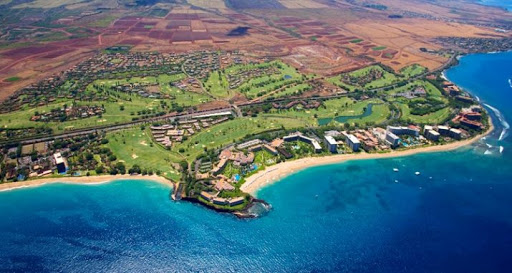
\includegraphics[width=1.0\paperwidth]{Maui.jpg}}
  \begin{frame}[plain]
  
\begin{mdframed}[tikzsetting={draw=black,fill=white,fill opacity=0.7,
               line width=0pt},backgroundcolor=none,leftmargin=20,
               rightmargin=20,innertopmargin=4pt]
\Huge County of Maui v. Hawaii Wildlife Fund
\end{mdframed}

  \end{frame}
}

%@@@@@@@@@@@@@@@@@@@@@@@@@@@@@@@@@@@@@@@@@@@@@@@@@
%\begin{frame}
%
%\begin{center}
%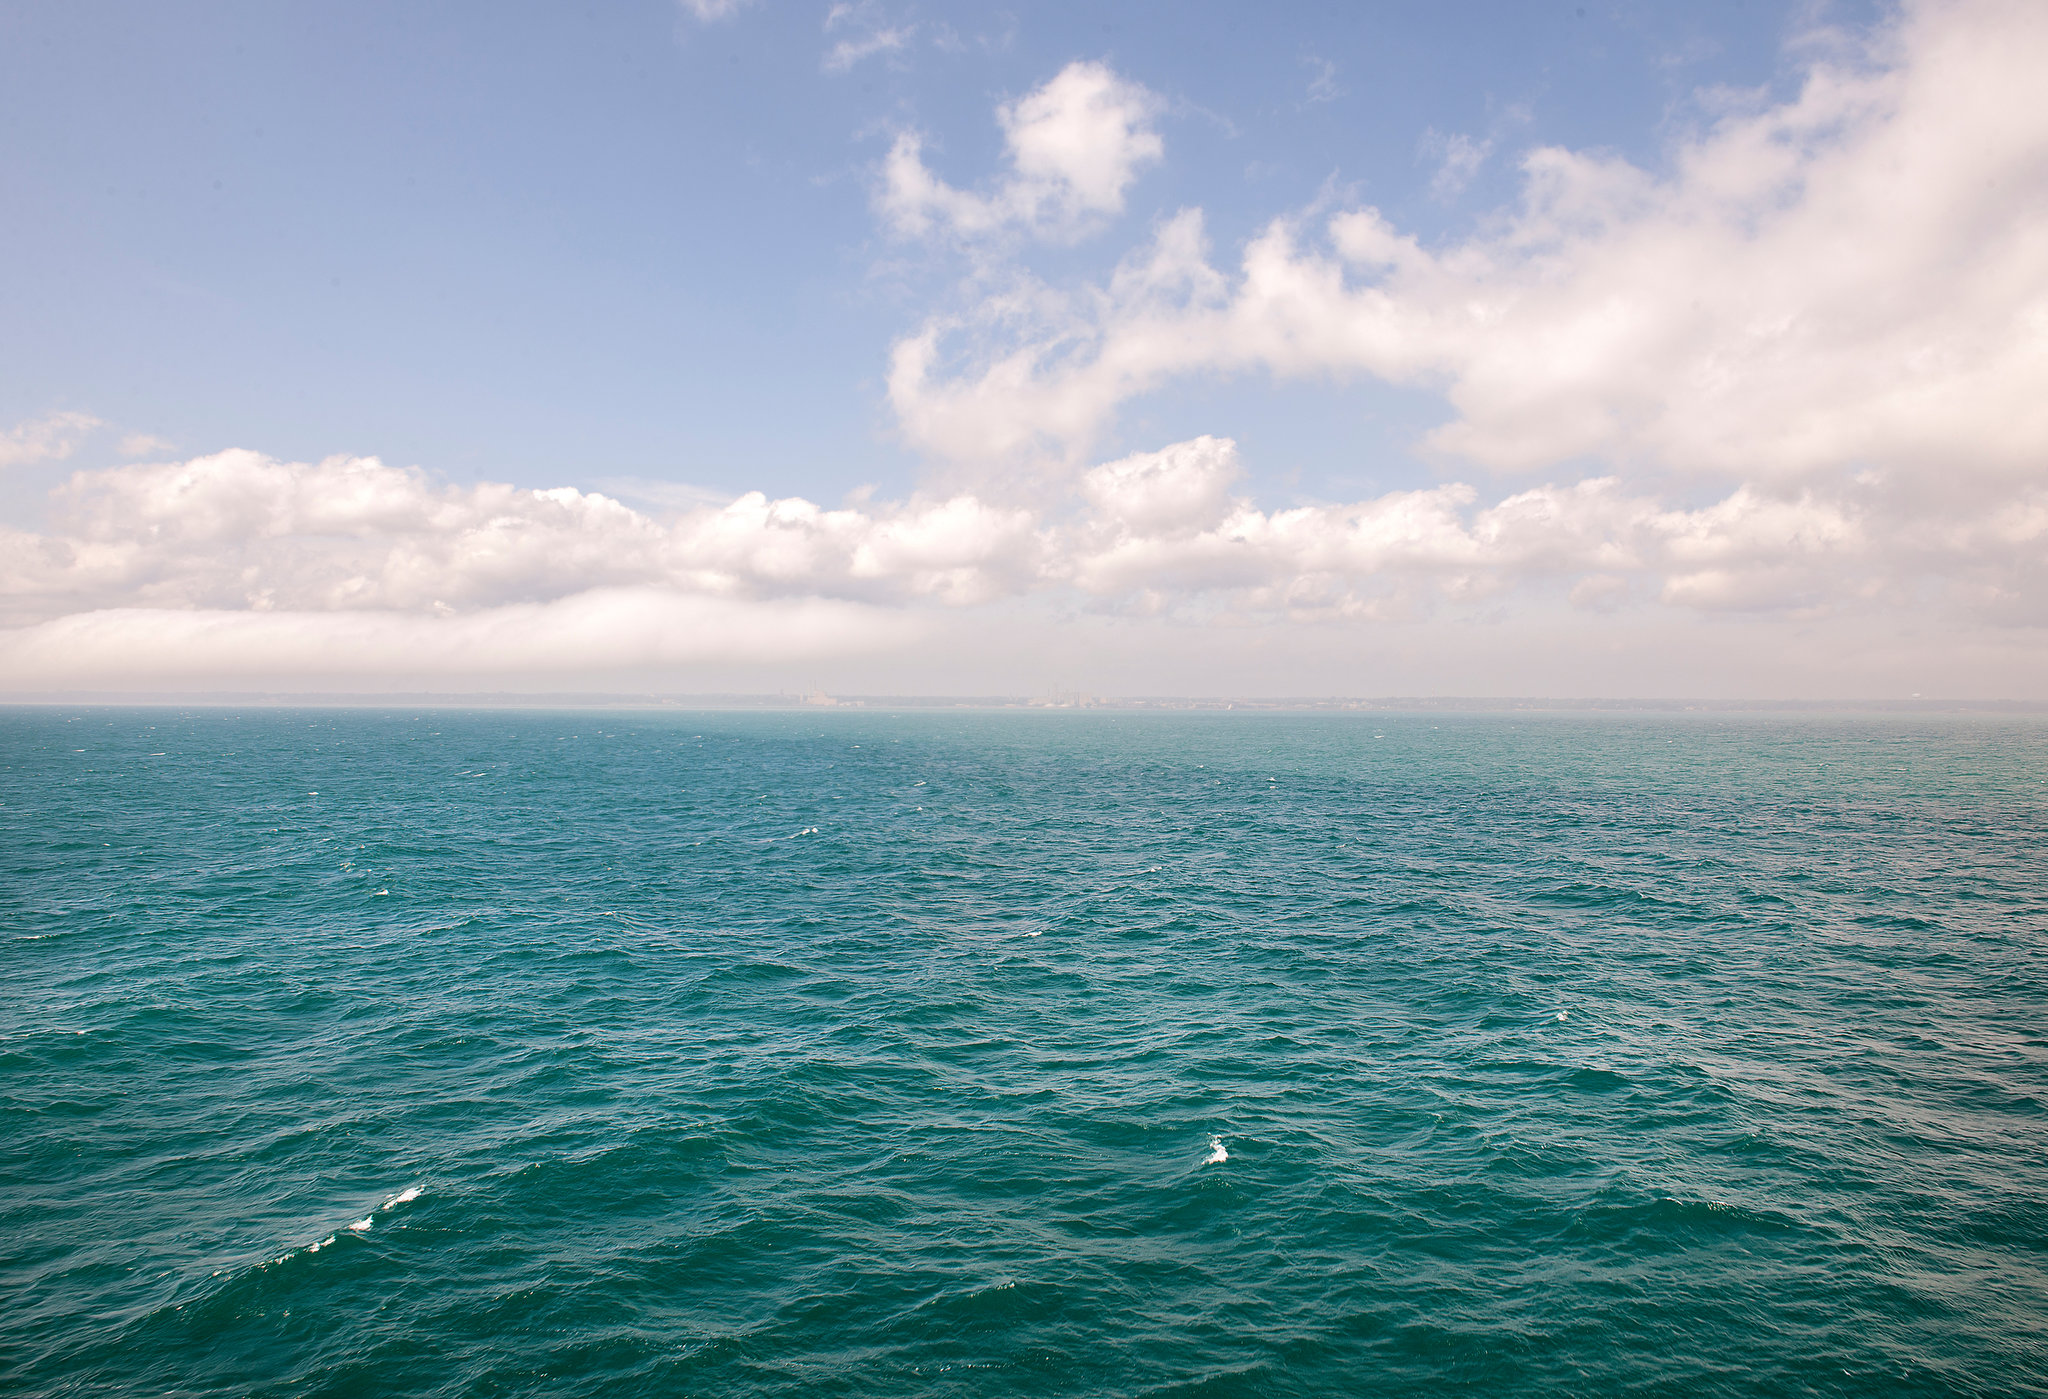
\includegraphics[scale=0.4]{lake_michigan.jpg}
%\end{center}
%
%
%\end{frame}

%@@@@@@@@@@@@@@@@@@@@@@@@@@@@@@@@@@@@@@@@@@@@@@@@@
\begin{frame}
\frametitle{Background: CWA}

\begin{itemize}

\item Developed and passed in response to national outrage over 1969 Cuyahoga River fire;
\bigskip
\bigskip
\item Very ambitious goals expressed in the CWA:
\begin{itemize}
\item `...discharge of toxic pollutants in toxic amounts be prohibited';
\item `...discharge of pollutants into the navigable waters be eliminated by 1985';
\item `...protection and propagation of fish, shellfish, and wildlife and provides for recreation in and 
on the water be achieved by July 1, 1983';
\item `...research and demonstration effort be made to develop 
technology necessary to eliminate the discharge of pollutants into the navigable waters':
\end{itemize}
\bigskip
\bigskip
\item Effect:
\begin{itemize}
\item Dramatic improvement in water quality;
\item Law lived up to potential... and is in need of reform.
\end{itemize}
\end{itemize}

\end{frame}

%@@@@@@@@@@@@@@@@@@@@@@@@@@@@@@@@@@@@@@@@@@@@@@@@@
\begin{frame}
\frametitle{Background: CWA}

\begin{itemize}

\item Covered: all waters `close to' navigable waters are covered by CWA;
\begin{itemize}
\item `waters of the United States, including the territorial seas';
\item Intermittent streams, dry lake beds, wetlands?
\item Rapanos v.United States: `...only those relatively permanent, standing or continuously flowing bodies of water...';
\end{itemize}
\bigskip
\item Point sources vs non-point sources;
\bigskip
\item Technology standards vs quality standards;
\bigskip
\item Tiered standards and anti-degradation;

\end{itemize}

\end{frame}

%@@@@@@@@@@@@@@@@@@@@@@@@@@@@@@@@@@@@@@@@@@@@@@@@@
\begin{frame}
\frametitle{Background: CWA -- six titles}

\begin{itemize}

\item Title I: declaration of goals, grants for R\&D;
\bigskip
\item Title II: construction grants for treatment facilities;
\bigskip
\item Title III: no discharge w/o permit, technology/quality standards;
\bigskip
\item Title IV: structure of permit program;
\bigskip
\item Title V: citizen suits, whistleblower protection;
\bigskip
\item Title VI: construction grants for treatment facilities, appended 1987;


\end{itemize}

\end{frame}

%@@@@@@@@@@@@@@@@@@@@@@@@@@@@@@@@@@@@@@@@@@@@@@@@@
\begin{frame}
\frametitle{Background: the case}
\begin{columns}

\begin{column}{0.5\textwidth}
\begin{itemize}

\item The Lahaina Wastewater Reclamation Facility (Maui County, Hawaii) treats wastewater from homes and businesses;
\bigskip
\item Authorized (EPA, Hawaii Department of Health) to inject the reclaimed water into four Class V wells on the island;
\bigskip
\item Leads to $\approx$3--5 million gallons/day of which $>$2.7--4.5 million gallons/day enters ocean via seepage;
\bigskip
\item EPA/state: no need for NPDES permit, not a \textbf{point source} under the CWA. 
\end{itemize}
\end{column}
%\begin{columns}

%\begin{column}{0.5\textwidth}
%TL;DR:
%\bigskip
%\begin{itemize}
%\item Egan part 1 documents a series of policy choices;
%\bigskip
%\item Those policy choices induced successive waves of ecological instability in the Great Lakes system;
%\end{itemize}
%
%\end{column}

%\onslide<1->
\begin{column}{0.5\textwidth}  %%<--- here
    \begin{center}
     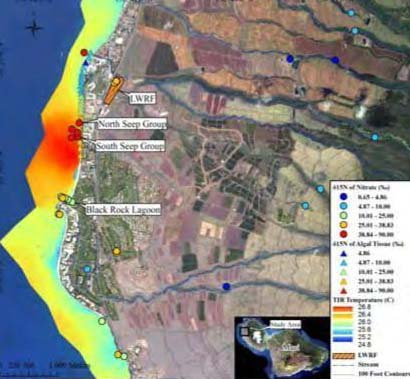
\includegraphics[scale=0.6]{a-tracer-dye.jpg}
     \end{center}
\end{column}

\end{columns}

\end{frame}

%@@@@@@@@@@@@@@@@@@@@@@@@@@@@@@@@@@@@@@@@@@@@@@@@@
\begin{frame}
\frametitle{Background}
\begin{columns}

\begin{column}{0.5\textwidth}

\begin{itemize}

\item University of Hawai‘i researchers put dye into wells --  able to trace wastewater;
\bigskip
\item Peak concentration of dye from wells 9-10 months later;
\bigskip
\item Estimated 64\% of wastewater in wells reaches ocean; treated wastewater could be as much as 92\% of spring output:
\bigskip
\item ``...our  results  conclusively  demonstrate  that a  hydrogeologic  connection  exists between LWRF Injection Wells 3 and 4 and the nearby coastal  waters of West Maui." 
\end{itemize}
\end{column}
%\begin{columns}

%\begin{column}{0.5\textwidth}
%TL;DR:
%\bigskip
%\begin{itemize}
%\item Egan part 1 documents a series of policy choices;
%\bigskip
%\item Those policy choices induced successive waves of ecological instability in the Great Lakes system;
%\end{itemize}
%
%\end{column}

%\onslide<1->
\begin{column}{0.5\textwidth}  %%<--- here
    \begin{center}
     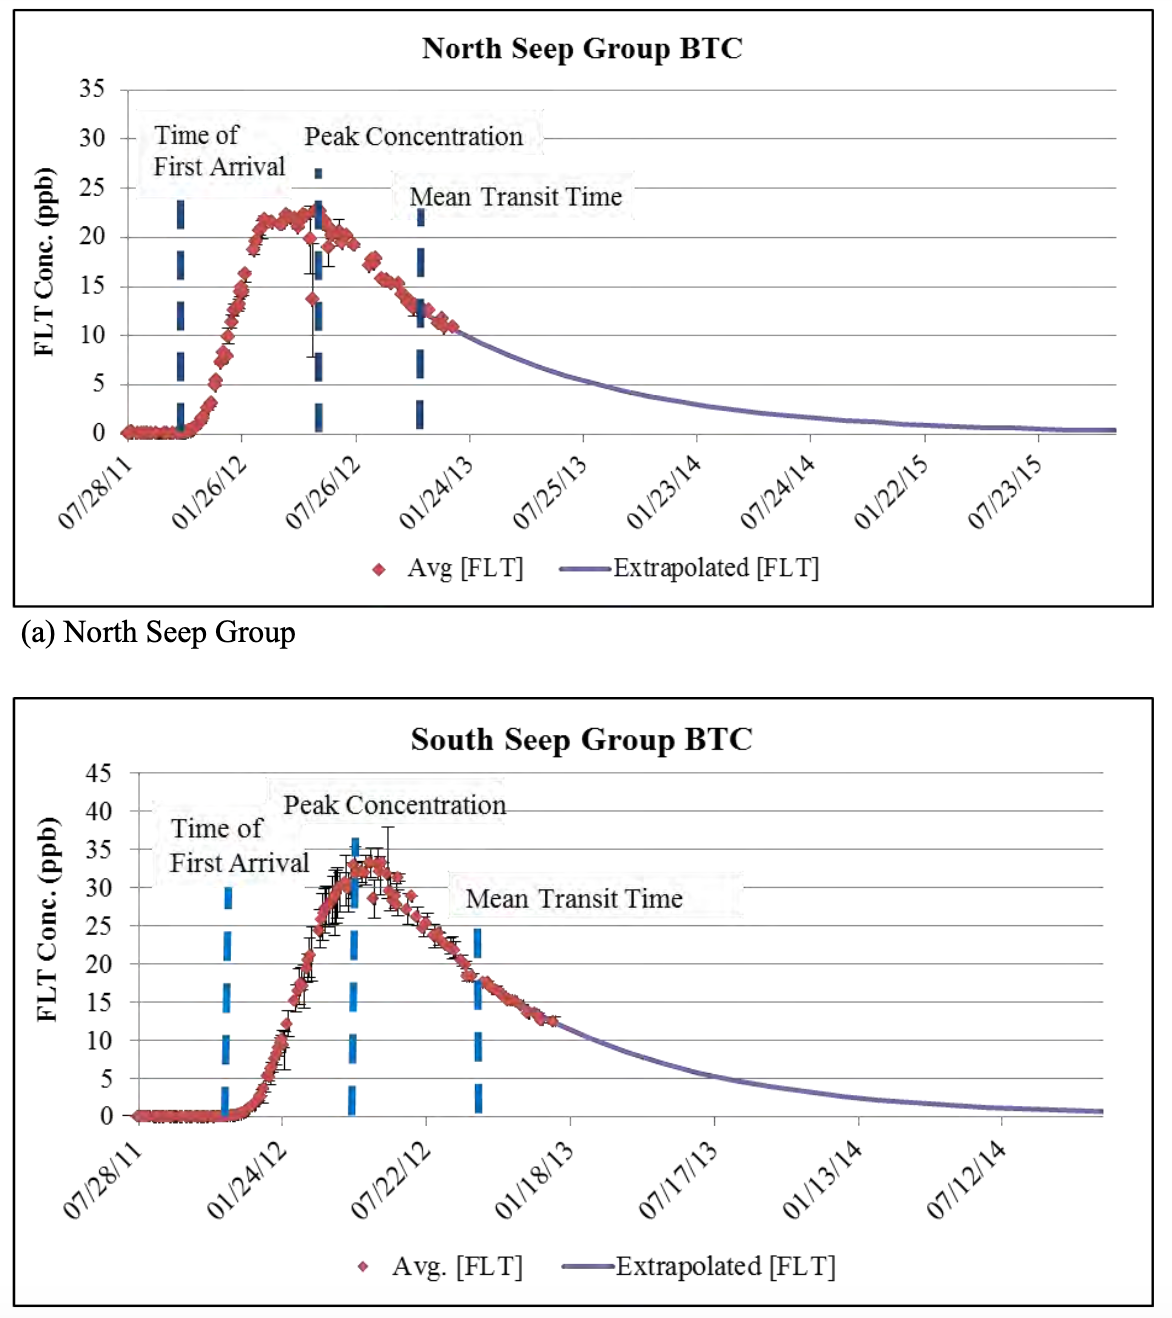
\includegraphics[scale=0.28]{dye_timing.png}
     \end{center}
\end{column}

\end{columns}
\end{frame}



%@@@@@@@@@@@@@@@@@@@@@@@@@@@@@@@@@@@@@@@@@@@@@@@@@
\begin{frame}
\frametitle{Background}

\begin{itemize}

\item After pleading with county to seek permitting for years, multiple environmental groups...
\begin{itemize}
\item Hawaii Wildlife Fund;
\item Surfrider Foundation;
\item Sierra Club-Maui;
\item Earthjustice;
\end{itemize}
sued the county for lacking permits;
\bigskip
\bigskip
\bigskip
\item EPA supported county, arguing that there was no need to permit under CWA.
\end{itemize}

\end{frame}


%@@@@@@@@@@@@@@@@@@@@@@@@@@@@@@@@@@@@@@@@@@@@@@@@@
\begin{frame}
\frametitle{Context: CWA}

\begin{center}
%\huge``...any addition of any pollutant to navigable waters from any point source..."\\
``\large 502(12) The term "discharge of a pollutant" and the term "discharge of pollutants" each means (A) any addition of any pollutant to navigable waters from any point source, (B) any addition of any pollutant to the waters of the contiguous zone or the ocean from any point source other than a vessel or other floating craft."\\
\bigskip
\Large\hspace{100mm}$\sim$CWA 1972
\end{center}

\begin{itemize}
\item Point sources that discharge to (necessarily "into" or "directly into"?) Waters of the United States require an NPDES permit;
\bigskip
\item Nonpoint sources are covered by separate policies (e.g., grants for farmers to manage runoff);
\end{itemize}

\end{frame}

%@@@@@@@@@@@@@@@@@@@@@@@@@@@@@@@@@@@@@@@@@@@@@@@@@
\begin{frame}
\frametitle{Context: CWA}

\begin{center}
\Large``The NPDES permit program, created in 1972 by the Clean Water Act (CWA), helps address water pollution by regulating point sources that discharge pollutants to waters of the United States. The permit provides two levels of control: technology-based limits and water quality-based limits (if technology-based limits are not sufficient to provide protection of the water body)."\\
\bigskip
\large\hspace{100mm}$\sim$https://www.epa.gov/npdes/about-npdes
\end{center}

\end{frame}

%@@@@@@@@@@@@@@@@@@@@@@@@@@@@@@@@@@@@@@@@@@@@@@@@@
\begin{frame}
\frametitle{Context: CWA}

\begin{center}
     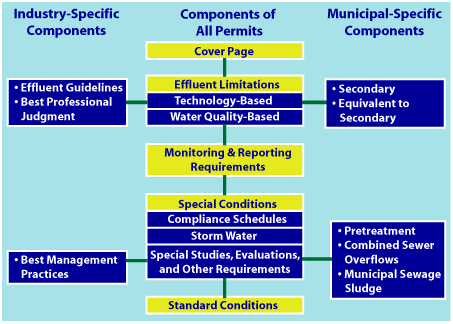
\includegraphics[scale=0.8]{NPDES_Permit_Components_EPA_chart.png}
\end{center}

\end{frame}

%@@@@@@@@@@@@@@@@@@@@@@@@@@@@@@@@@@@@@@@@@@@@@@@@@
\begin{frame}
\frametitle{Context: legalese}

\begin{itemize}
\item statutory provision, structure, interpretation
\item interpretive guidance
\item deference
\item citizen suit
\item cert. (certiorari)
\item plaintiff, respondent, Solicitor General, amici briefs
\item textual argument (textualism vs. originalism)
\item bright line
\item proximate cause 
\item judgment to reverse/affirm
\item majority, plurality, dissent, dicta
\item settle
\end{itemize}
\end{frame}

%@@@@@@@@@@@@@@@@@@@@@@@@@@@@@@@@@@@@@@@@@@@@@@@@@
\begin{frame}
\frametitle{First Decision}

\begin{itemize}
\item In 2014 United States District Court for the District of Hawaii found for plaintiffs: facility needed NPDES permits;
\bigskip
\bigskip
\item Healdsburg test: plaintiffs must demonstrate a hydrologic connection between the aquifer and the ocean (that is ``direct and immediate");
\begin{itemize}
\item need a connection;
\item connection needs to matter;
\end{itemize}
\end{itemize}
\end{frame}

%@@@@@@@@@@@@@@@@@@@@@@@@@@@@@@@@@@@@@@@@@@@@@@@@@
\begin{frame}
\frametitle{Second Decision}

\begin{itemize}
\item County appealed - appeals for United States District Court for the District of Hawaii go to Ninth Circuit;
\bigskip
\item In 2018 Ninth Circuit found for plaintiffs: held that CWA required a permit if pollutants are ``fairly traceable" to original point source;
\bigskip
\item Traceability test: drew on Rapanos v. United States;
\begin{itemize}
\item A 4-1-4 split;
\item Four justices for ``do nothing" and let stand the ``hydrological connection" test;
\item Justice Kennedy for a new (more limited?) "significant nexus" test;
\item Four justices for a new (much more limited) "permanent surface waters only" test;
\item Kennedy joined the ``surface waters only" justices in judgement/outcome (ruling for Mr. Rapanos) but did not join their opinion, making it a plurality opinion not a majority opinion and thus not precidental--i.e., not binding policy. 
\end{itemize}
\end{itemize}
\end{frame}

%@@@@@@@@@@@@@@@@@@@@@@@@@@@@@@@@@@@@@@@@@@@@@@@@@
\begin{frame}
\frametitle{Second Decision}

    \begin{center}
     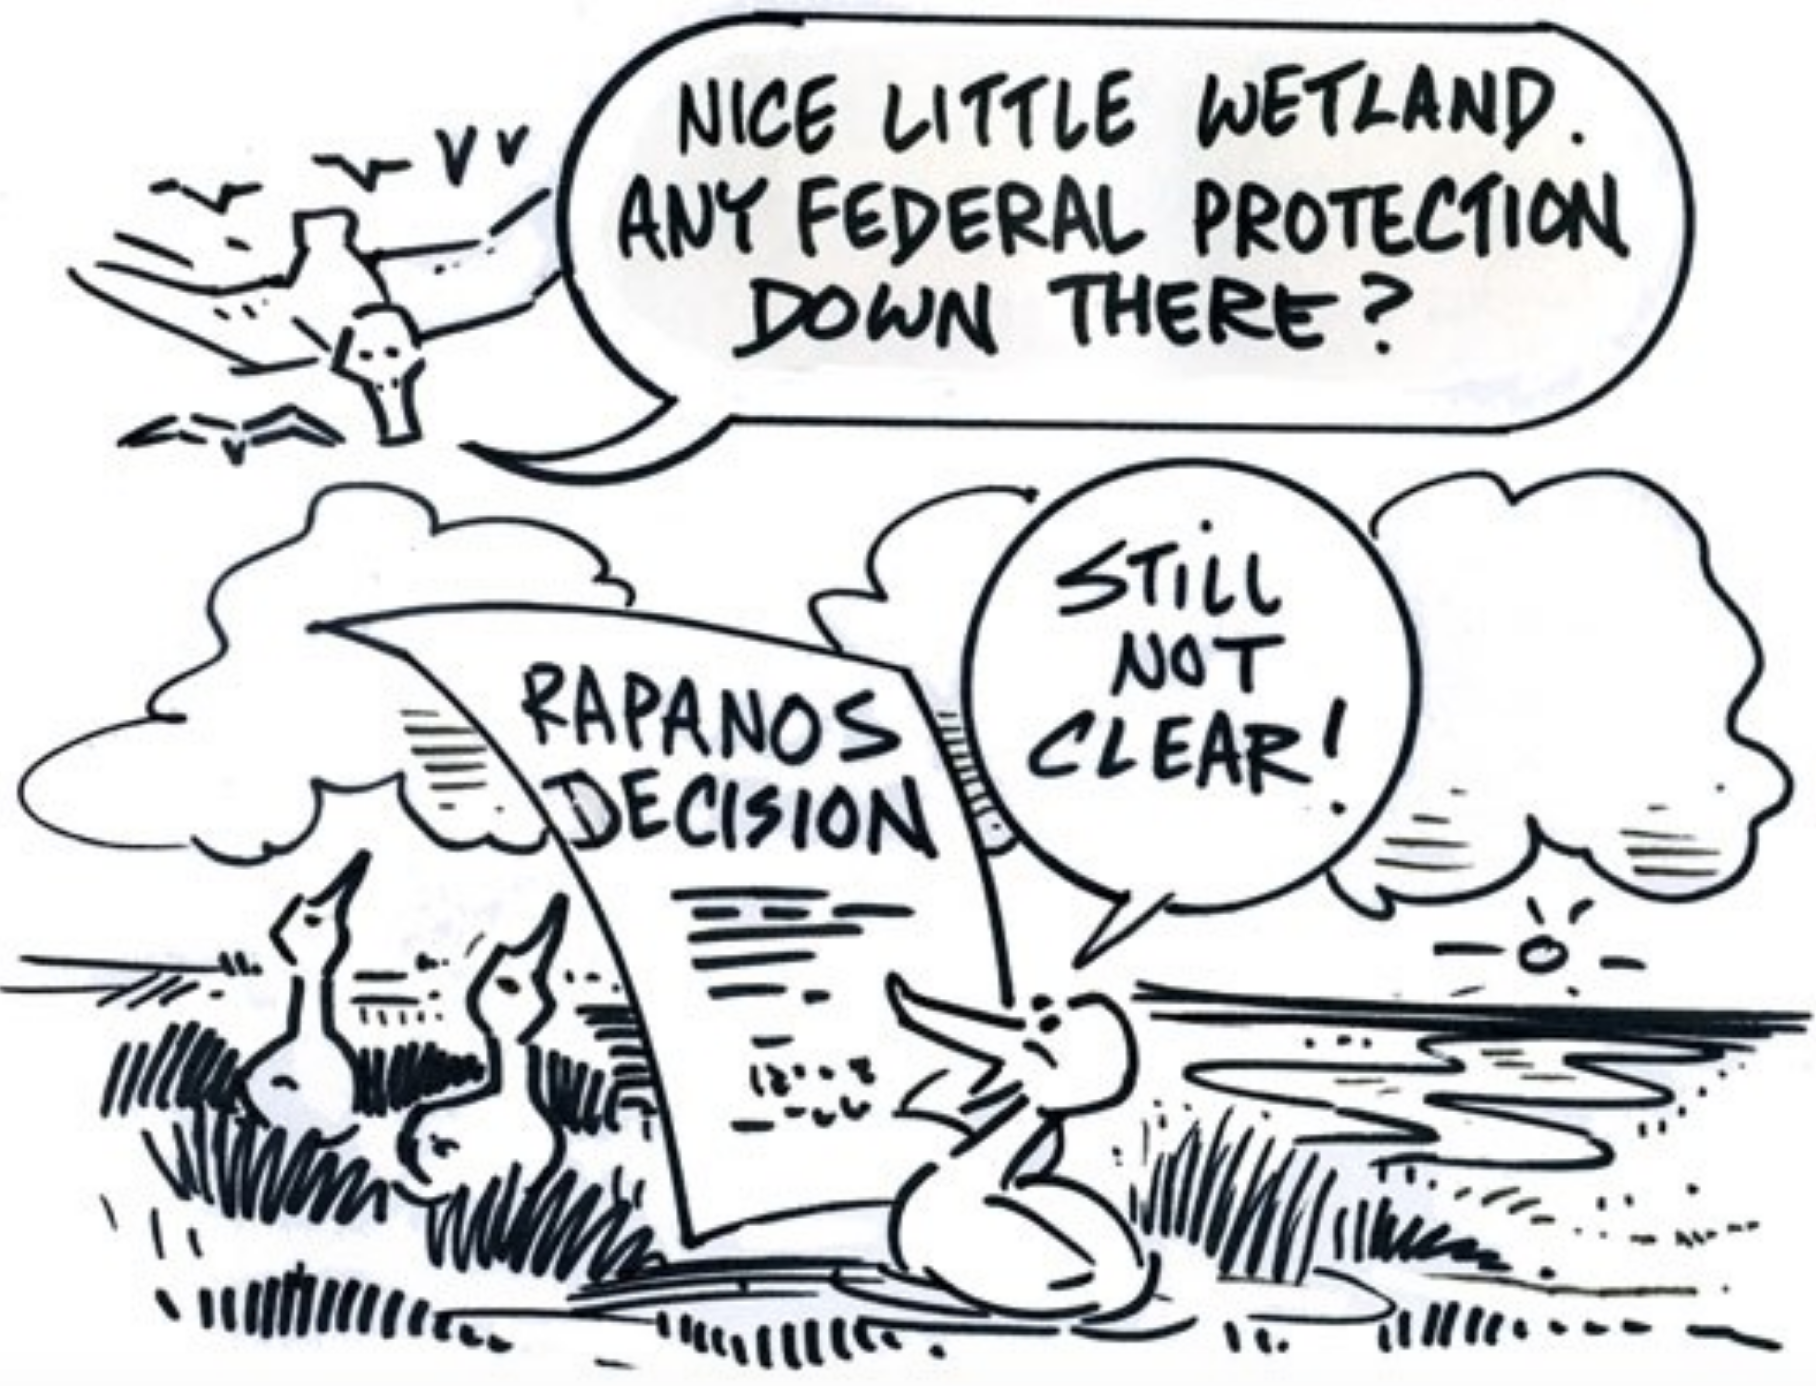
\includegraphics[scale=0.28]{rapanos.png}
     \end{center}

\end{frame}

%@@@@@@@@@@@@@@@@@@@@@@@@@@@@@@@@@@@@@@@@@@@@@@@@@
\begin{frame}
\frametitle{So what were they left with?}

\begin{itemize}
\item A decision that relied on a precidentially ambiguous judgement;
\bigskip
\bigskip
\item Advanced an novel, possibly ambiguous test -- no bright line?;
\bigskip
\bigskip
\item EPA changed positions to be more in line with county;
\bigskip
\bigskip
\item County filed for writ of certiorari to the Supreme Court.
\end{itemize}
\end{frame}

%@@@@@@@@@@@@@@@@@@@@@@@@@@@@@@@@@@@@@@@@@@@@@@@@@
\begin{frame}
\frametitle{Third Decision}

\begin{itemize}
\item Parties agree that: 
\begin{itemize}
\item treated waste water is a pollutant;
\item wells are point sources;
\item ocean is navigable;
\item groundwater is not a point source;
\end{itemize}
\bigskip
\item Parties disagree about ``from";
\begin{itemize}
\item County argued that ``from" means ``delivered by";
\item Plaintiff argued that ``from" means ``starting point";
\end{itemize}
\bigskip
\item 30 amicus briefs: 
\begin{itemize}
\item EPA: groundwater is excluded - breaks causal chain;
\item Solicitor general: supports EPA’s position - no agency deference to EPA requested;
\end{itemize}
\end{itemize}
\end{frame}

%@@@@@@@@@@@@@@@@@@@@@@@@@@@@@@@@@@@@@@@@@@@@@@@@@
\begin{frame}
\frametitle{Third Decision}

\begin{itemize}
\item Vacated the Ninth Circuit decision;
\bigskip
\item Breyer: Permit required for point sources or for non-point sources when there is ``the functional equivalent of a direct discharge";
\bigskip
\item Functionally equivalent to direct discharge test:
\begin{itemize}
\item distance pollutant travels from point source to waterway;
\item time;
\end{itemize}
\bigskip
\item Case remanded to Ninth Circuit under instructions to consider Functionally equivalent to direct discharge test.
\end{itemize}
\end{frame}


%@@@@@@@@@@@@@@@@@@@@@@@@@@@@@@@@@@@@@@@@@@@@@@@@@
\begin{frame}
\frametitle{Final Thoughts}

\begin{itemize}
\item Why did we listen to this?
\bigskip
\bigskip
\item Demonstration of the complexity of putting policy into law (e.g. ``from");
\bigskip
\bigskip
\item Reminder that the Supreme Court does not ONLY declare things constitutional or not - they are final arbiter of statutory interpretation;
\bigskip
\bigskip
\item \textbf{Is the Clean Water Act good?}

\end{itemize}

\end{frame}



\end{document}








